\chapter{Introduction}

For hundreds of years, newspapers inform the public and hold the powerful accountable. Two things contributed to its establishment. First, the invention of the printing press by Johannes Gutenberg was a technological catalyst. The flow of information was immensely increased. Before, writings such as books had to copied by writing each single page by hand. Second, the enlightenment spurred the critical reflection of power structures. But for the longest time in history, the communication in a newspaper was unidirectional. The journalists wrote their articles and the readers had to consume them. Nevertheless, the writing and their political implications were discussed in a smaller circles. For instance in the 19th century, the bourgeoisie organized in reading societies as portrayed by the painter Johann Peter Hasenclever in Figure~\ref{fig:lesegesel}.

\begin{figure}[h]
	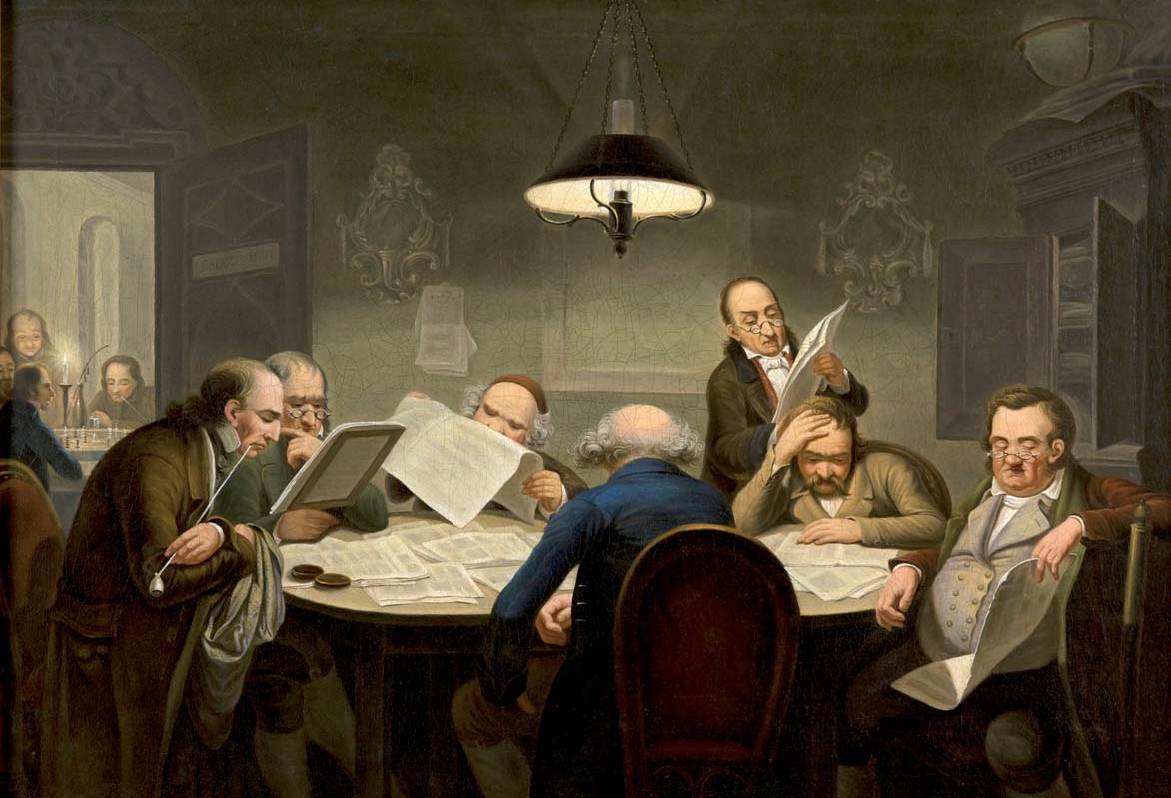
\includegraphics[width=1\textwidth]{images/intro/Lesegesellschaft.png}
	\caption[Caption for LOF]{Johann Peter Hasenclever: \textit{Das Lesekabinett} (The Reading Society), 1843.\protect\footnotemark}
	\label{fig:lesegesel}
\end{figure}

\footnotetext{\url{https://commons.wikimedia.org/wiki/File:Lesegesellschaft,_um_1843.png}}

The audience is limited when discussing an issue in person. A way for a non-journalist to join the debate in a newspaper are \textit{letters to the editor}. Everybody can send their opinions in a letter to the editors of newspapers. Editors can then decide to print a selection. Until today, this is a common tool for newspapers to give voice to the ordinary people. However, it is rather unlikely that the letters are printed since space in a printed newspaper is sparse.
The introduction of the Web revolutionized media. News are now delivered online as well and the space restrictions of the Internet are more relaxed.
Since the era of so called \textit{Web 2.0}, users generate content themselves.
These developments established the \textit{comment section} as a special place on blogs, social media platforms or newspapers where users can leave their thoughts.

Figure~\ref{fig:nyt_article_comment} displays two typical comments on an opinion piece of the New York Times.

\begin{figure}[h]
\begin{tabular}{ll}
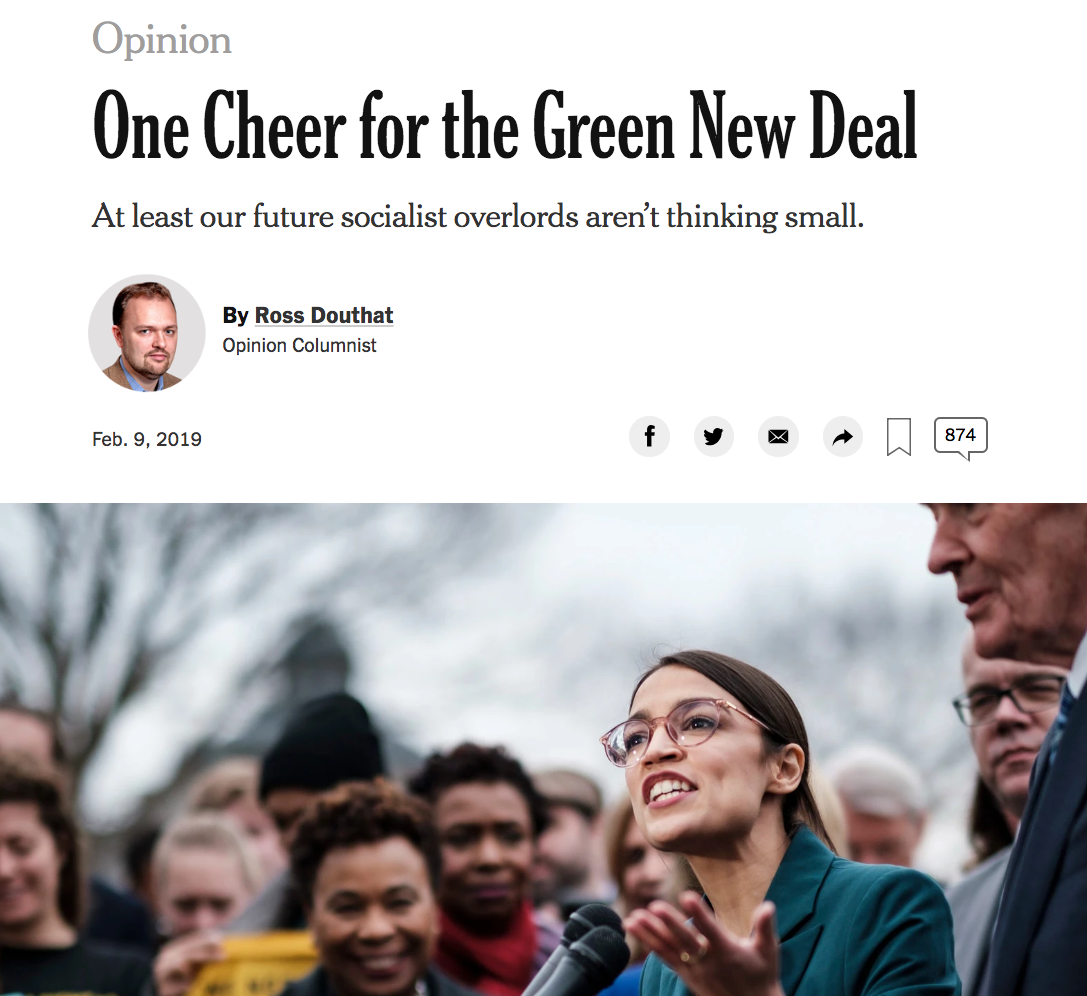
\includegraphics[width=0.6\textwidth]{images/intro/nyt_article.png}
&
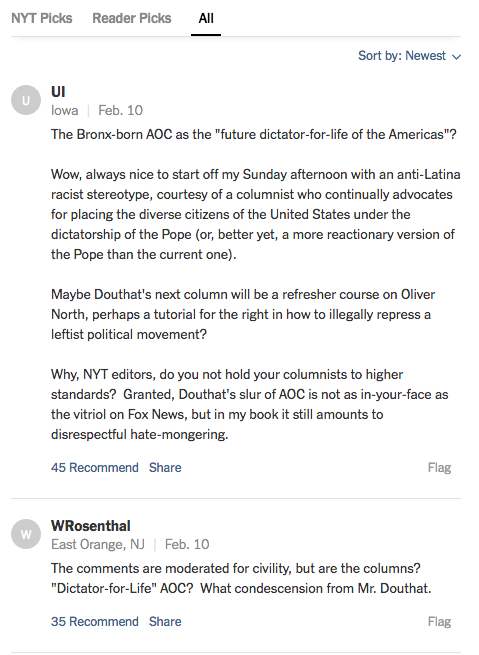
\includegraphics[width=0.4\textwidth]{images/intro/nyt_comment1.png}
\end{tabular}
\caption[Caption for LOF]{An option article of the New York Times received 878 comments before the comment section was closed.\protect\footnotemark}
\label{fig:nyt_article_comment}
\end{figure}

\footnotetext{\url{https://www.nytimes.com/2019/02/09/opinion/alexandria-ocasio-cortez-green-new-deal.html}}

In the beginning, comments were hailed as a democratization of the debate. In contrast to the previous unidirectional communication, the communication is now multidirectional. Readers can discuss an article with one another. They can also give new perspectives to an issue by contributing personal stories or adding expert knowledge on a specific subject. Furthermore, they hold journalists accountable as Glenn Greenwald\footnote{\url{https://theintercept.com/2017/12/18/comments-coral-project/}} states:

\begin{quote}
``Journalists often tout their responsibility to hold the powerful accountable. Comments are a way to hold journalists themselves accountable.''
\end{quote}

In addition, the introduction of online news comments was an emancipatory act of depriving journalists of their role as gatekeepers. For the first time, a debate was open for everybody with an Internet connection -- so almost everybody. This sets the idea of discourse ethics as proposed by J{\"u}rgen Habermas into practice.
The essence of this thought is the belief, that a collective by exchanging arguments can come to superior conclusions than a sole person.
This is a stark contrast to the prior philosophical idea of Immanuel Kant's categorical imperative which focuses on individuals' convictions. The concept of Habermas is vague and implementation-agnostic but there are certain rules to follow. One rule, i.e., declares that arguments must not be repeated. And he promises if all participants obey the rules, the community will eventually reach a common conclusion which then manifests the morale. So in the best case, readers discuss an issue under an article and in the end, all participants share the same opinion.
Nevertheless, this in an idealistic scenario and Habermas did not have news comments in mind when he developed the idea in the beginning of the 1970s.
In the following, we examine the current problems of news comments and show that repeated arguments may not the biggest one.

\begin{figure}[h]
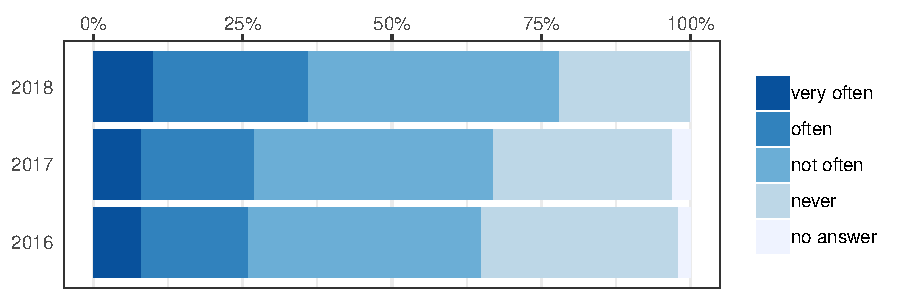
\includegraphics[width=1\textwidth]{graphs/hate_on_the_web/hate_paper.pdf}
\caption[Caption for LOF]{"Have you witnessed hate speech or hast posts on the Internet?". This question is part of a survey among 1000 Germans by the \textit{Landesanstalt Medien NRW}.\protect\footnotemark}
\label{Fig:hate_on_the_web}
\end{figure}

\footnotetext{\url{https://www.medienanstalt-nrw.de/fileadmin/user_upload/lfm-nrw/Foerderung/Forschung/Dateien_Forschung/forsaHate_Speech_2018_Ergebnisbericht_LFM_NRW.pdf}}

Online news outlets are drowning in the vast quantity of user comments. While there are certainly high-quality comments that follow the high hopes of emancipation, there are also comments which are rather unwelcome. They range from out-of-topic discussions to the use of offensive language. A survey by the \textit{Landesanstalt Medien NRW} among German Internet users is shown in Figure~\ref{Fig:hate_on_the_web}. The survey reveals that users increasingly witness hate on the Web. To remove problematic comments, the comment section needs to be moderated. But the moderation process involves specially trained humans who decide about the existence of comments. Consequently, newspapers abolish their comment section altogether. The biggest German daily newspaper, \textit{Sueddeutsche Zeitung}, closed their comment section in 2014 as one of the earliest newspaper\footnote{\url{https://www.freitag.de/autoren/jan-jasper-kosok/die-sz-schliesst-ihre-kommentarfunktion}}.

In 2016, a survey\footnote{\url{https://netzpolitik.org/2016/umfrage-zeitungsredaktionen-schraenken-kommentarfunktionen-2015-weiter-ein/}} among German news outlets showed that two in five restricted commenting on their website.
Although moderators could help, they are expensive and the news industry already has economic problems and is on a decline.
In Figure~\ref{fig:decline_of_newspapers}, two graphs illustrate the problem on the example of the US news sector. The number of employees was almost cut by half from 2004 to 2017. In mid 2000s, the advertising revenue decreased rapidly. One reason are ad-blocking tools for users to hide advertisement to increase the overall user experience. Another reason are new, strong competitors in the online advertising market. The Internet enables new and more creative forms of advertisement with, e.g., Google's AdWords or influencers on Instagram.
The news sector is in a ambivalent state.
While recent technological development allows novel ways of storytelling with, i.e., interactive graphics, decreasing revenue streams, that go along with it, remain an open problem.
Solving it is out of scope of this master's thesis but Natural-Language Processing (NLP) using machine learning techniques promises to improve efficiency in managing news comments.
As a consequence, less manual moderation is required so the comment sections remain open which fosters our democracy.

\begin{figure}
    \centering
    \subfloat[Employees in the US news sector.\protect\footnotemark]{{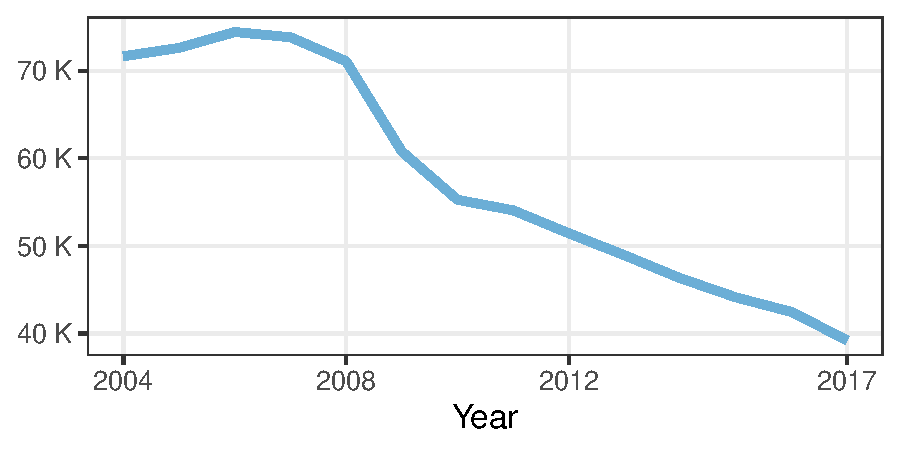
\includegraphics[width=0.5\textwidth]{graphs/decline_of_newspapers/emp_paper.pdf} }}
    \subfloat[Revenue in the US news sector.\protect\footnotemark]{{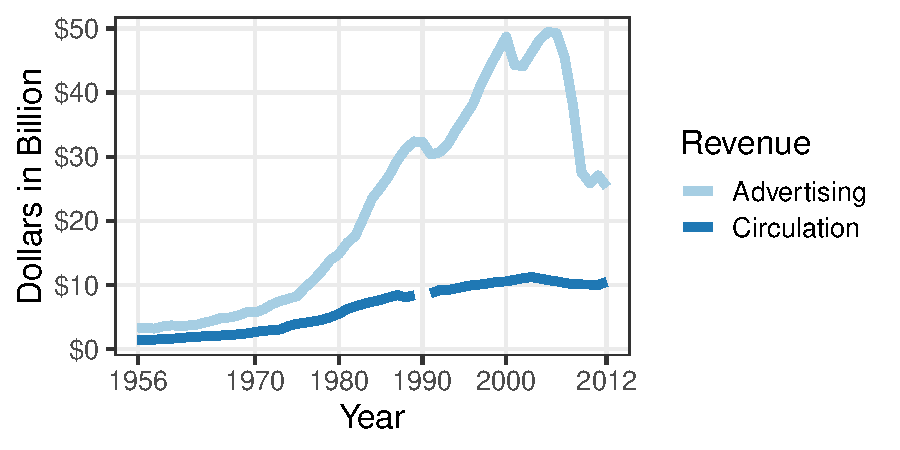
\includegraphics[width=0.5\textwidth]{graphs/decline_of_newspapers/rev_paper.pdf} }}
    \caption{The decline of the US news sector at the example of number of employees and revenue.}
    \label{fig:decline_of_newspapers}
\end{figure}

\footnotetext{Source: Pew Research Center analysis of Bureau of Labor Statistics Occupational Employment Statistics data.}
\footnotetext{Source: News Media Alliance, formerly Newspaper Association of America (through 2012); Pew Research Center analysis of year-end SEC filings of publicly traded newspaper companies (2013-2017).}

 There already exist works to automatically detect hate speech or abusive language in user-generated content~\cite{hateoffensive, Nobata:2016:ALD:2872427.2883062, risch_delete_nodate, schmidt2017survey}. In this work, we focus on classifying comments in a more general way.
Comments are assigned to different categories. For instance, what the sentiment of a comment is or whether it is off-topic.
It can be any criteria for classification.
This classification can aide comment moderators and also creates new opportunities for other features. For instance, comments are currently mainly ranked chronologically or based on their up- and down-votes. The classification of comments allows to rank them by specific criteria. A feature which is enabled by classification are comment filters. One could choose to hide a specific kind of comments. This is already in production on social media platforms such as Twitter or Facebook. They automatically hide low quality or unpleasant comments. With a fine-grained comments classification, one could think of even more possibilities. For example, a user is tired of negativity and only wants to read comments with a positive sentiment.

In contrast to prior work, we assume that the article's context, namely, the whole conversation, is essential to make a classification of a single comment. The article acts as a conversation-starter and the comments leading up to the comment are the conversation partners. To illustrate our motivation, we take two humanly-annotated comments from a Canadian newspaper~\cite{kolhatkar2018sfu}:

\begin{quote}
    ``Time for the elders and chiefs to stand up to the plate and take a leadership role!''
 \end{quote}

This comment is labeled as constructive (or in other words: high-quality) and
\begin{quote}
    ``Maybe this will motivate the cabbies in TO to clean their filthy cars! That are a disgrace.''
\end{quote}

is labeled as non-constructive. For humans, it is hard to make a judgment without reading the corresponding article and previous comments first. Moreover, the annotators were required to read the article first before deciding whether an article is constructive. So we should be fair and also give the machine the possibility to obtain the context before classifying.
The term `context' describes different aspects in this domain.
One could also think of context by considering a commentator's previous comment history.
While this would probably help to improve the performance of a classifier, it is unfair.
A classification of text should depend only on a very comment.
We illustrate this differentiation using following example.
In a fair judicature, a conviction must be based on clear evidence not on the criminal history.
The history only matters for determining the sentence.
This should apply for the classification of comments as well: only the current text is important, neither previous comments nor misbehavior.
Also from a privacy perspective it is important to point out, that creating information about users means profiling them.
Storing personal information has further implications since they are under severe protection with the European Union General Data Protection Regulation (GDPR) in force.
It is recommended to only store personal information when it is absolutely necessary.
For this work, we do not use any user information for classification.

In order to formally define the problem of conversation-aware classification, let $C$ and $A$ be the set of all comments and articles respectively.
In addition, we define:
\\\\
$\text{isArticle}=\{(c, a)| \forall (c,a) \in C \times A: c\text{ is a comment of }a\}$
\\
$\text{isPrevious}=\{(c, o, a)| \forall (c,o, a) \in C \times C \times A:\text{isArticle(}c, a\text{)} \wedge \text{isArticle(}o, a\text{)} \wedge \\  c_{time} > o_{time}\}$

The training set $T =\{(c_n, a_n, s_n, y_n)\}^N_{n=1}$ consists of quadruple-wise data, where $c \in C$, $a \in A$, $s \subseteq \{o | \forall o \text{ isPrevious(}c,o,a)\}$ and $(c, a) \in \text{isArticle}$.
Further, $y \in Y $ is the corresponding label for $Y=\{1,\dotsc, l\}$ classes.
We wish to train a classifier $\gamma$ that maps a comment, its article, and its previous comments (in the conversation) to classes: $\gamma: C \times A \times C^* \rightarrow Y$.

The field of journalism is tightly coupled with the technological advancement of our society. As mentioned earlier, only through the printing press could humans spread information so fast. This allowed the journalistic profession to establish and flourish. The ongoing digital revolution also affects journalists and there is a long tradition of supporting their work with digital technologies. It started in the late 1960s with computer-assisted reporting and lead to current ideas about automatic reporting. Right now, there is a larger effort by supporting newspapers in managing their user comments. On example is the unprecedented Coral Project\footnote{\url{https://coralproject.net}}, a cooperation among Mozilla, the New York Times, and the Washington Post, that interviewed more than 400 experts in 150 newsrooms to develop an IT system to manage comments. Research on news comments or other user-generated content is done extensively in other research fields. For instance, there exists research on news comments in the field of communication studies. Recent work by Ksiazek and Springer~\cite{eldridge_ii_user_2018} gives an overview over current trends and future directions in this area. The increasing hate in the comment section is one object of investigation. Besides, there is a multitude of publications that highlight the importance of a comment's context. Loosen et al.~\cite{loosen_making_2017} formulated several comment quality indicators after conducting interviews with news professionals as well as developing a software mockup. Among other things, they list `reference to the article' and `references to other comments' as an indicator for high-quality comments. Their work is built upon earlier research done by Diakopoulos et al.~\cite{Diakopoulos:2011:TQD:1958824.1958844} and Noci et al.~\cite{noci2012comments} who also investigate characteristics of comments. The relation of one comment to other comments or the article itself plays a role when looking at the perception of comments. There is also an abundance of comment guidelines that describe comments that newspaper desire. The New York Time writes in their guidelines\footnote{\url{https://help.nytimes.com/hc/en-us/articles/115014792387-Comments}}: ``We are interested in articulate, well-informed remarks that are relevant to the article.'' Also, the community guidelines by the Guardian requires commentators to ``keep it relevant''\footnote{\url{https://www.theguardian.com/community-standards}}.
So, the relation of comment to the article and previous comments is important to consider. Machine learning methods ought to respect the knowledge generated in non-computer-science fields and try to include them into their own work.

This thesis is structured as follows. In Section~\ref{ch:related_work}, we give a detailed overview of related scientific work before providing background information in Section~\ref{ch:background}.
In Section~\ref{ch:datasets}, we describe the datasets we conduct experiments on.
In Section~\ref{ch:approach}, we present our contributions and evaluate them in Section~\ref{sec:evaluation}.
Finally, we conclude in Section~\ref{chp:conclusions} and give an outlook for future work.

